\documentclass{article}
\usepackage{commands, biblatex, subcaption, pgfplots}
\addbibresource{sources.bib}
\usepackage{titlesec}
\usepackage[margin=1in]{geometry}
\newcommand{\V}{\mathbb V}
\newcommand{\I}{\mathbb I}
\pgfplotsset{compat=1.18}
\title{\textsc{\Large{Bridging Algebra and Geometry: Hilbert's Nullstellensatz}}}
\author{Timothy Cho}
\date{December 2023}

\begin{document}
\maketitle
\begin{abstract}
Hilbert's Nullstellensatz gives a bijection between a specific subset of polynomial ring ideals and geometric objects describable by algebraic equations. In this paper, we give intuition on this fundamental theorem through examples from both the algebraic and geometric viewpoints. We describe the concepts of \textit{variety} and \textit{ideal}, which are maps in opposing directions between the set of ideals in a polynomial ring over a field $k[x_1,\ldots, x_n]$ and the collection of subsets of $k^n$ which are solutions to systems of polynomial equations. In this paper, we prove that the variety and ideal maps are invertible in one direction but not the other. However, we will state and prove Hilbert's Nullstellensatz, which shows that while this second direction is not fully invertible, we are, in an algebraically closed field $k$, able to restrict the domain of ideals in $k[x_1,\ldots, x_n]$ we discuss in order to get a useful bijection.
\end{abstract}

\titleformat{\section}[block]{\normalfont\scshape\filcenter}{\thesection. }{0pt}{}

\section{Introduction}
Algebra arose from people finding ways to solve polynomial equations. Linear and quadratic polynomials were well-understood since antiquity, and polynomials of degrees $3$ and $4$ were the topic of intense study in 16th-century Europe \cite{waerden}. In the same vein, the work of Niels Henrik Abel (1802-1829) and his contemporaries showed that there was no general solution in radicals to polynomial equations of degree at least $5$. While it seemed as if this branch of algebra was ``closed off" to further mathematical exploration, this work led to the development of rigorous abstract algebra.

We can continue to chase abstraction by considering \textit{systems} of polynomial equations instead: given a set $S\subseteq k[x_1, \ldots, x_n]$, where $k$ is a field, what is the common set of roots to every polynomial in $S$? The case that every $f\in S$ had degree $1$ led to the modernization of linear algebra, from which arose our definitions of \textit{vector spaces} and \textit{subspaces}, which abstracted and generalized the visual notions of lines and planes that we are accustomed to in two- and three-dimensional Euclidean space.

This type of generalization is the heart of algebraic geometry: we ask for the common set of roots $V$ given a set $S\subseteq k[x_1, \ldots, x_n]$, except now each $f\in S$ can take any degree. Moreover, we pose an inverse question: given a set of ``solutions" $V\subseteq k^n$ ($n$-dimensional space over a field $k$), what are all of the polynomials that vanish on $V$? That is, we would like to encode spatial, geometric information as algebraic information (a set of polynomials), and vice versa. Algebraic geometry is the study of this ``translation manual" between algebra and geometry; however, as with language, translation manuals could never produce a bijective correspondence. In many cases, two distinct sets of polynomials $S, T\subseteq k[x_1, \ldots, x_n]$ can share a vanishing set $V$. This is potentially disastrous; however, in 1893, David Hilbert (1862-1943) proved the Nullstellensatz in a paper on invariant theory, an area of mathematics closely related to modern algebraic geometry. The Nullstellensatz states that, in an algebraically closed field, the way objects are ``lost in translation" is quite predictable: $S$ and $T$ as above are always essentially ``synonymous" with each other, so that we can safely disregard a large portion of subsets of $k[x_1, \ldots, x_n]$ to get a useful bijection.

As such, algebraic geometry exploded over the 20th century --- instead of a weak link between shapes and polynomials, the modernization of algebra along with the bridge of Hilbert's Nullstellensatz allowed mathematicians to express shapes through rigorously-defined rings and ideals. This partially allows us to do away with the need of visuals, in favor of abstraction and generalization. Thus, objects which may seem nonsensical, like a ``curve" in $\F_9^2$ (2-dimensional space over the field of $9$ elements), suddenly become meaningful, and even relevant. As a result, modern algebraic geometry continues to reveal previously-unseen connections between areas of mathematics, and today, algebraic geometry intersects with almost every branch of mathematics that is studied \cite{smith}.

To give an example of a problem solved by algebraic geometry, one need not consider further than Fermat's Last Theorem, which states that there do not exist positive integers $a,b,c$ such that $a^n + b^n = c^n$, where $n\geq 3$. This conjecture is ostensibly not very geometric. However, by building off of work in algebraic geometry and number theory, Andrew Wiles (1953-) converted the problem into a statement about {curves} and successfully proved the conjecture in 1994. More generally, ideas in number theory are usually represented algebraically, but algebraic geometry provides useful alternative viewpoints.

In Section 2, we provide the ring theoretic background needed for the proof of the Nullstellensatz. In Section 3, we introduce the \textit{variety} and \textit{ideal}, the two main objects of study in algebraic geometry, and we provide examples and graphs for certain varieties (Example \ref{algvarexamples}). We also note a few basic propositions about varieties and ideals, and suggest that they are nearly mutually inverse. Finally, in Section 4, we build towards a proof of Hilbert's Nullstellensatz (Theorem \ref{nullstellensatz}) via Noether's Normalization Lemma (Theorem \ref{noether}) and applying Rabinowitsch's Trick from the so-called ``weak" form of the Nullstellensatz (Theorem \ref{weak}).

\section{Algebraic Preliminaries}
All rings in this paper are unital and commutative, so all ideals are automatically two-sided. Also, if $R$ is a ring and $I\subseteq R$ is an ideal, for clarity we will write $I\furina R$ in lieu of $I\subseteq R$. Finally, whenever we have an inclusion of rings $R\leq S$, we will assume $1_R = 1_S$.
\\

We start by generalizing the familiar concept of roots of polynomials.
\begin{definition}\label{root}
Let $R$ be a ring, and let $f\in R[x_1, \ldots, x_n]$. A \textit{root} of $f$ is an $n$-tuple $a = (a_1, \ldots, a_n)\in R^n$ such that $f(a) = f(a_1, \ldots, a_n) = 0$.
\end{definition}

If $R = k$ is a field, then any $f \in k[x]$ has at most $\deg f$ distinct roots, so the set of roots of $f$ is finite. However, our next example demonstrates that root-finding is far more interesting in multiple variables.

\begin{example}\label{x^2+4y^2-4}
Let $f(x):= (x^2+4y^2-4)^2\in \R[x,y]$, and let $V$ be the set of roots of $f$. If $a := (x,y)\in V\subseteq \R^2$, then $f(a) = 0$ if and only if $x^2+4y^2=4$. Hence, $V = \{(x,y)\in \R^2: x^2+4y^2=4\}$. To gain a geometric perspective, we divide by $4$ go obtain $(x/2)^2+ y^2 = 1$. Hence, we can visualize $V$ is an ellipse centered at the origin, with semimajor axis $2$ and semiminor axis $1$: 
\begin{figure}[h!]
    \centering
    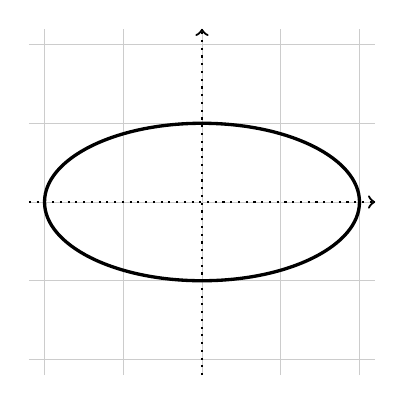
\begin{tikzpicture}
        \draw[very thin, color=black!20] (-2.2,-2.2) grid (2.2,2.2);
        \draw[->, dotted, thick] (-2.2, 0) -- (2.2,0);
        \draw[->, dotted, thick] (0, -2.2) -- (0,2.2);
        \draw[very thick] (0,0) ellipse (2 and 1);
    \end{tikzpicture}
    \caption{$V = \{(x,y): x^2+4y^2=4\}$.}
    \label{ellipse}
\end{figure}
\end{example}

From the previous example, we expect that it is usually the case that multivariate polynomials have infinite sets of roots. Now, we pose an related question central to algebraic geometry: given a polynomial ring $k[x_1, \ldots, x_n]$ and a set $V\subseteq k^n$, how do we easily describe the set of polynomials that share $V$ as a common set of roots? The language of rings and ideals will do nicely here. However, to understand an ideal, we should understand its generating set. Hence, we introduce the definition below.
\begin{definition}
A ring $R$ is \textit{Noetherian} if every ideal $I\furina R$ is finitely generated.
\end{definition}

\begin{example}
The ring $\Z$ is a PID. Hence, $\Z$ is Noetherian, as every ideal $I\furina \Z$ is generated by one element.
\end{example}

The next result, proved by Hilbert in 1890, allows us to quickly see if a polynomial ring is Noetherian.
\newpage

\begin{theorem}[Hilbert Basis Theorem] \label{hilbertbasis}
Let $R$ be a ring. If $R$ is Noetherian, so is $R[x]$.
\end{theorem}
See \parencite[Theorem 3.11]{maliar} for a proof in full detail; we provide a sketch below. 
\begin{proof}[Proof Sketch]\renewcommand{\qedsymbol}{$\bullet$}
Suppose $R$ is Noetherian. If $I\furina R[x]$ is an ideal, we find that $J$, the set of all leading coefficients of polynomials in $I$, is an ideal of $R$. Let $J = \gen A$, where $|A|<\infty$. Now, for each $a\in A$, select a polynomial $g\in I$ with leading coefficient $a$, and let $G\subseteq R[x]$ be the set of all such $g$'s chosen. By finiteness, $G$ has a polynomial of maximal degree $k$. 

Now, for each degree $i\leq k$, let $J_i\furina R$ be the ideal consisting of the leading coefficients of polynomials in $I$ with degree at most $i$. Hence for each $i\leq k$, pick a finite generating set $A_i$ with $J_i = \gen{A_i}$, and pick $G_i$ similar to above. Define $I_0 := \gen{G, G_0, G_1, \ldots, G_k}\furina R[x]$. By construction, $I_0$ is finitely generated, and $I_0\subseteq I$. To show that $I\subseteq I_0$, suppose for contradiction that there exists some $f\in I\setminus I_0$ of minimal degree. From here, casework on the degree of $f$ shows a contradiction, so $I = I_0$; hence $R[x]$ is Noetherian.
\end{proof}

By induction, we have the following corollary.
\begin{corollary}\label{noetheriancorollary}
Let $R$ be a ring. If $R$ is Noetherian, so is $R[x_1, \ldots, x_n]$.
\end{corollary}

Hence, all of the rings we will encounter in this paper will be Noetherian. An important example of a non-Noetherian ring would be a polynomial ring $R[x_1, x_2, \ldots]$, with infinitely many indeterminates $x_i$, but we will not consider it in this paper except in this short comment.
\\

Our next definition will occur frequently in the examples of Section 3, and it is used in the statement of Hilbert's Nullstellensatz (Theorem \ref{nullstellensatz}).
\begin{definition}\label{radical}
Let $R$ be a ring and $I\furina R$. The \textit{radical of $I$} is the set
$$\sqrt{I} := \left\{r\in R: r^n \in I \textrm{ for some } n\in \Z^+\right\}.$$
Similarly, $I\furina R$ \textit{is radical} if $I = \sqrt I$.
\end{definition}
Informally, $\sqrt I$ is the set of all ``$n$th roots" of elements of $I\furina R$. It is readily checked that $I\subseteq \sqrt I$, and with some work one can show $\sqrt I\furina R$. Although computing radicals given an arbitrary $I$ is usually not an easy task, it is manageable if $I$ is principal. We give two examples.

\begin{example}\label{radcomputation}
Let $I := \gen{(x^2+4y^2-4)^2}\furina \Z[x,y]$. If $f\in \sqrt I$, then $f^n \in \gen{(x^2+4y^2-4)^2}$ for some $n\in\Z^+$. Observe that $x^2+4y^2-4\in \sqrt I$. Moreover, we can check that $x^2+4y^2-4$ is irreducible, so we claim that ${\sqrt I = \gen{x^2+4y^2-4}}$. Indeed, if $f\in \gen{x^2+4y^2-4}$, then $f = g(x,y)(x^2+4y^2-4)$ for some $g(x,y)\in\Z[x,y]$, so that $f^2 = g(x,y)^2(x^2+4y^2-4)^{2} \in I$. Hence $f\in \sqrt I$ and $\gen{x^2+4y^2-4}\subseteq \sqrt I$.

For the reverse inclusion, fix $f\in\sqrt I$, so there exists some $n\in\Z^+$ such that $f^n\in I$. Taking $V$ as defined in Example \ref{x^2+4y^2-4}, we see that $f^n$ vanishes on $V$. But this is only possible if $x^2 + 4y^2 = 4$, so that $f$ has an irreducible factor of $x^2+4y^2-4$. Hence $f\in \gen{x^2+4y^2-4}$, so $\sqrt I = \gen{x^2+4y^2 - 4}$.
\end{example}

\begin{example}
We give a example of a radical $I\furina \Z[x]$. Let $I := \gen{x^2 - 2x+2}\furina \Z[x]$. If $f\in\sqrt I$, then $f^n\in \gen{x^2-2x+2}$ for some $n\in\Z^+$. However, $x^2-2x+2$ is quadratic and has no integer roots, so it is irreducible. Thus, we claim $\sqrt I = \gen{x^2 - 2x+2} = I$, and the proof of this is similar to the argument in the previous example.
\end{example}

From above, notice that since the polynomial $x^2-2x+2$ is irreducible, $\gen{x^2-2x+2}$ is a prime ideal. However, we also saw that the ideal was radical, and this is in fact true in general: when $I\furina R$ is prime, no work is needed to assert $\sqrt I = I$.

\begin{proposition}\label{primeradical}
Prime ideals are radical.
\end{proposition}
\begin{proof}
Let $R$ be a ring and $I\furina R$ be prime. We know $I\subseteq \sqrt I$, so fix $r\in \sqrt I$. By well-ordering, there exists some \textit{minimal} $n\in\Z^+$ such that $r^n\in I$. If $n=1$, we are done, so suppose $n\geq 2$. Write $r^n = rr^{n-1}$, but because $I$ is prime, $r\in I$ or $r^{n-1}\in I$. Assume $r\not\in I$. Then $r^{n-1} \in I$, but this violates the minimality of $n$, a contradiction. Hence $r\in I$, so $\sqrt I\subseteq I$ and thus $I=\sqrt I$.
\end{proof}

Finally, we review two basic definitions from ring theory. The first of these is related to the various notions of \textit{integrality} we will see in Definition \ref{integrality}, which we will use to prove the Nullstellensatz.
\begin{definition}
Let $R\leq S$ be an inclusion of rings. An element $s\in S$ is \textit{algebraic} over $R$ if $s$ is the root of some $f(x)\in R[x]$. If $s\in S$ is not algebraic, then $s$ is \textit{transcendental} over $R$.
\end{definition}

Although we give a generalized definition here, we will be purely discussing algebraicity over integral domains, rather than arbitrary rings.
\\

Our final definition is a critical assumption needed for Hilbert's Nullstellensatz to hold.
\begin{definition}
A field $k$ is \textit{algebraically closed} if every non-constant polynomial $f\in k[x]$ has a root in $k$.
\end{definition}

\section{A Geometric Perspective}
With our algebraic tools in place, we return to our main discussion on polynomial roots. Recall the set $V$ from Example \ref{x^2+4y^2-4}, which described an ellipse in $\R^2$. Before we give a general definition, we first examine a simpler example: visualizing the roots of a polynomial in one variable.

\begin{example}\label{1dim}
The set of roots $V$ of $x^4-5x^2  +4 \in \R[x]$ is $\{\pm 1, \pm 2\}$. On the real number line, we visualize $V$ as follows:
\begin{figure}[h!]
\centering
\begin{tikzpicture}
\draw[->] (-5.5,0) -- (5.5,0);
\draw \xtick{-5};\draw\xtick{-4};\draw \xtick{-3};\draw \xtick{-2};\draw \xtick{-1}; \draw\xtick{0};\draw\xtick{1};
\draw\xtick{2};
\draw\xtick{3};
\draw\xtick{4};
\draw\xtick{5};
\draw (0, -0.2) node[anchor=north]{0};
\draw (5, -0.2) node[anchor=north]{5};
\draw (-5,-0.2) node[anchor=north]{$-5$};
\draw (5.6, -0.2) node[anchor=north]{$\R$};
\filldraw[fill=black] (1, 0) circle (0.1);
\filldraw[fill=black] (2, 0) circle (0.1);
\filldraw[fill=black] (-1, 0) circle (0.1);
\filldraw[fill=black] (-2, 0) circle (0.1);
\end{tikzpicture}
\caption{A one-dimensional algebraic variety.}
\label{1D}
\end{figure}
\end{example}
Figure \ref{1D} above is a very simple example of an \textit{algebraic variety}, which, informally, is the ``visualization" of the roots of a polynomial, or of a set of polynomials. Varieties are profoundly boring in one dimension: given any $f\in k[x]$ (where $k$ is a field), the variety of $f$ has at most $\deg f < \infty$ points. However, our discussion will focus on polynomials in multiple variables; hence, we give our main, general definition below.

\begin{definition}\label{variety}
Let $k$ be a field and $S\subseteq k[x_1, \ldots, x_n]$. The \textit{affine algebraic variety of $S$} is the set of common roots of all of the polynomials in $S$:
$$\V(S) := \left\{a\in k^n: f(a) = 0\textrm{ for all } f\in S\right\}.$$
Similarly, $V\subseteq k^n$ is an \textit{algebraic set} if $V = \V(S)$ for some $S\subseteq k[x_1, \ldots, x_n]$.
\end{definition}
We note that there are other types of varieties beyond affine varieties; see \cite{smith}. However, in the scope of this paper, all varieties will be affine, so we write ``variety" when we mean ``affine algebraic variety."

\begin{example}\label{algvarexamples}
The following are examples of varieties.
\begin{enumerate}
\item In Example \ref{x^2+4y^2-4}, we found that in $\R^2$, $\V\paren{(x^2+4y^2-4)^2}$ is an ellipse.\footnote{We dropped the set brackets in the notation here for convenience --- we do this whenever it does not cause confusion.}
\item Let $f(x,y) := x^2+y^2-4$ and $g(x,y) := x-1$, where both polynomials are viewed as being in $\R[x,y]$. Then $\V(fg)$ is the set $\{(x,y): (x^2+y^2-4)(x-1) = 0\}$, which consists of the circle centered at the origin of radius 2 and the vertical line $x=1$. We also see that $\V(fg) = \V(f)\cup \V(g)$: the visualization for this is found in Figure \ref{sub1}.
\item Let $f,g$ be as above, and let $h(x,y) := y-1$. Then $\V(fg, fh)$ is the set of points in $\R^2$ that vanish on both $fg$ and $fh$; which, by solving a system of equations, we see that $\V(fg, fh)$ consists of the point $(1,1)$ and the circle centered at the origin of radius $2$. Notice that this is precisely the intersection $\V(fg,fh) = \V(fg) \cap \V(fh)$: see Figure \ref{sub2}.
\item Any point in $\R^3$ can be viewed as an algebraic variety. Indeed, if $(a,b,c)\in \R^3$, then $\{(a,b,c)\} = \V(x-a, y-b, z-c)$. Generalizing this, if $k$ is any field, then any point in $k^n$ is viewable as an algebraic variety: if $(a_1, \ldots, a_n) \in k^n$, then $\{(a_1,\ldots, a_n)\} = \V\paren{\{x_i-a_i\}_{i=1}^n}$.
\item Generalizing the previous point, if $k$ is a field, we can show that any finite subset of $k^n$ is an algebraic set. This is similar to the one-dimensional case we discussed in Example \ref{1dim}.
\item An \textit{elliptic curve} in $\R^2$ is a set of points satisfying the equation $y^2=x^3+ax+b$ for some $a,b\in\R$, where $4a^3+27b^2\neq 0$. It is easy to see that if $C$ is an elliptic curve, then $C = \V(x^3-y^2 + ax +b)$. Elliptic curves are important in number theory, cryptography, as well as many other branches of mathematics. Andrew Wiles applied the theory of elliptic curves, which rests on algebraic geometry, to prove Fermat's Last Theorem \cite{smith}. An example of an elliptic curve is given in Figure \ref{sub3}.
\end{enumerate}
\end{example}
\begin{figure}[h!]
    \hspace{1 cm}
    \begin{subfigure}{0.30\textwidth}
    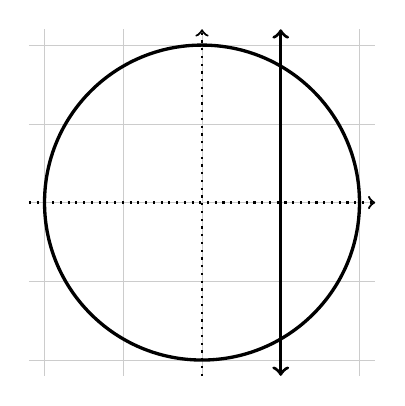
\begin{tikzpicture}
    \draw[very thin, color=black!20] (-2.2, -2.2) grid (2.2, 2.2);
    \draw[dotted, ->, thick] (-2.2,0) -- (2.2, 0);
    \draw[dotted, ->, thick] (0,-2.2) -- (0, 2.2);
    \draw[very thick] (0,0) circle (2);
    \draw[very thick, <->] (1,-2.2) -- (1, 2.2);
    \end{tikzpicture}
    \caption{$\V\brak{(x^2+y^2-4)(x-1)}$}
    \label{sub1}
    \end{subfigure}
    \hfill
    \begin{subfigure}{0.30\textwidth}
    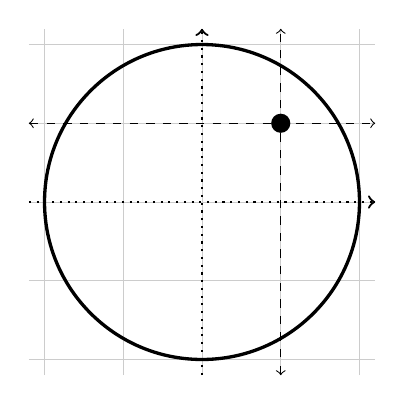
\begin{tikzpicture}
    \draw[very thin, color=black!20] (-2.2, -2.2) grid (2.2, 2.2);
    \draw[dotted, ->, thick] (-2.2,0) -- (2.2, 0);
    \draw[dotted, ->, thick] (0,-2.2) -- (0, 2.2);
    \draw[dashed, <->] (1, -2.2) -- (1, 2.2);
    \draw[dashed, <->] (-2.2, 1) -- (2.2, 1);
    \draw[very thick] (0,0) circle (2);
    \filldraw[very thick] (1, 1) circle (0.10);
    \end{tikzpicture}
    \caption{$\V(fg, fh) = \V(fg) \cap \V(fh)$}
    \label{sub2}
    \end{subfigure}
    \hfill
    \begin{subfigure}{0.30\textwidth}
    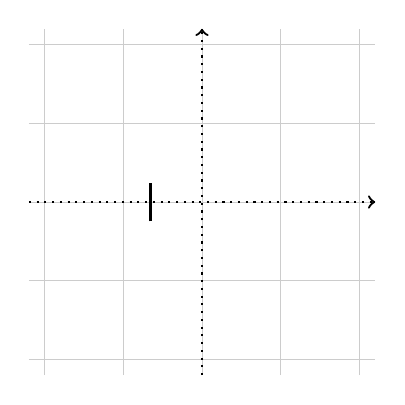
\begin{tikzpicture}[domain=-0.75:1.33]
    \draw[very thin, color=black!20] (-2.2, -2.2) grid (2.2, 2.2);
    \draw[dotted, ->, thick] (-2.2,0) -- (2.2, 0);
    \draw[dotted, ->, thick] (0,-2.2) -- (0, 2.2);
    \draw[very thick, ->] plot[id=top] function{sqrt(x * x * x + x + 1)};
    \draw[very thick, ->] plot[id=bot] function{-1 * sqrt(x*x*x+x+1)};
    \draw[very thick] (-0.657, -0.246) -- (-0.657, 0.246);
    \end{tikzpicture}
    \caption{$\V(x^3-y^2+x+1)$}
    \label{sub3}
    \end{subfigure}
    \caption{Various algebraic varieties as described in Examples \ref{algvarexamples}(2), (3), and (6).}
    \label{the big fig}
\end{figure}

Our reasoning in Examples \ref{algvarexamples}(2) and (3) can be generalized into the proof of the following proposition, which we exclude for brevity.
\begin{proposition}\label{unionintersection}
Let $k$ be a field and $S, T \subseteq k[x_1, \ldots, x_n]$. Then $\V(S)\cup \V(T) = \V(ST)$, and $\V(S)\cap \V(T) = \V(S\cup T)$, where $ST := \{f\cdot g: f\in S, g\in T\}$.
\end{proposition}

\begin{remark}\label{inclusionflip}
From Proposition \ref{unionintersection}, we should be quick to notice that the operation of ``taking the variety" flips the inclusion: if $S\subseteq T$, then $\V(S\cup T) = \V(T) = \V(S)\cap \V(T)$, which implies $\V(T)\subseteq \V(S)$. This is consistent with our intuitions, as it should be more ``difficult" for a point in $k^n$ to be a common zero for a larger set of polynomials $T$ compared to a smaller set $S$. As such, we mention here that unsurprisingly, we will see that the bijection of Hilbert's Nullstellensatz also flips the inclusion.
\end{remark}

As we have seen, varieties convert lists of polynomials into subsets of $k^n$. However, it is natural to consider the dual notion: given a subset $V\subseteq k^n$, what is the \textit{set of polynomials} that vanish on all of $V$?

\begin{example}\label{1dideal}
Refer back to Example \ref{1dim}, where we found the roots of $x^4-5x^2+4\in \R[x]$. However, we now fix the set of roots $V = \{\pm 1, \pm 2\}$, and ask for the set of all polynomials that vanish on $V$. We know that $f(x) := x^4-5x^2+4$ vanishes on $V$, but more generally, if $g\in \R[x]$, then $fg$ also vanishes on $V$, though it may vanish on more roots than just the four listed in $V$. However, it is clear that the polynomials in $\gen{x^4-5x^2+4}\furina \R[x]$ all vanish on \textit{at least} $V$.
\end{example}

This motivates our next definition.

\begin{definition}\label{ideal}
Let $k$ be a field, and let $V\subseteq k^n$. The \textit{ideal of $V$} is the set of all polynomials in $k[x_1, \ldots, x_n]$ that vanish on all of $V$:
$$\I(V) := \set{f\in k[x_1,\ldots, x_n]: f(a) = 0 \textrm{ for all } a\in V}.$$
\end{definition}
Immediately, we should notice a similarity between Definitions \ref{variety} and \ref{ideal}: all we have done was switch the roles of $k[x_1, \ldots, x_n]$ and $k^n$, in a manner we will make precise with Proposition \ref{revnull} and the Nullstellensatz (Theorem \ref{nullstellensatz}). For now, it is relatively safe to conjecture that due to this role exchange, the operations $\V$ and $\I$ are mutually inverse. We view a two-dimensional example of an ideal.

\begin{example}\label{idealcomputation}
With respect to Example \ref{x^2+4y^2-4}, let $V = \{(x,y): x^2 + 4y^2 = 4\}\subseteq \R^2$. Then $\I(V)$ is the set of polynomials in $\R[x,y]$ that vanish on $V$. Clearly, $x^2+4y^2-4\in \I(V)$, and if $f\in \R[x,y]$ is any polynomial, $f(x,y)(x^2+4y^2-4)\in \I(V)$. Hence, given this ``absorption property," we claim that $\I(V) = \gen{x^2+4y^2-4}$. We have demonstrated the inclusion $\I(V)\supseteq \gen{x^2 +4y^2-4}$ above. If $\I(V)\not\subseteq \gen{x^2+4y^2-4}$, there exists a polynomial $f\in \I(V)\setminus \gen{x^2+4y^2-4}$. Now, $f$ vanishes on $V$, so $f(x,y)$ must satisfy $x^2+4y^2 = 4$. If $(x^2+4y^2-4) \mid f$, this shows $f\in \gen{x^2+4y^2-4}$, so we assume $f\mid (x^2+4y^2-4)$, so $\deg f = 1$. However, we can check that $x^2+4y^2-4$ is irreducible, so such an $f$ cannot exist. Hence $\I(V) = \gen{x^2+4y^2-4}$.
\end{example}

In the example above, $\I(V)$ was actually an ideal in the ring-theoretic sense. Indeed, it is for this reason that mathematicians chose the name ``ideal" for this subset:
\begin{proposition}
Let $k$ be a field and $V\subseteq k^n$. Then $\I(V) \furina k[x_1, \ldots, x_n]$.
\end{proposition}
\begin{proof}
By definition, $\I(V) \subseteq k[x_1, \ldots, x_n]$. Take $f, g\in \I(V)$, and fix $a\in V$. Then $f(a) = g(a) = 0$, so $(f-g)(a) = f(a) - g(a) = 0$, so $f - g \in \I(V)$. Hence, $(\I(V), +) \leq (k[x_1, \ldots, x_n], +)$. Now, we check the absorption property. Take $f\in \I(V)$, $r\in k[x_1, \ldots, x_n]$, and fix $a\in V$. Since $f(a) = 0$, it follows that $rf(a) = r(a) \cdot f(a) = r(a)\cdot 0 = 0$, so $rf\in \I(V)$. Hence $\I(V)$ is an ideal.
\end{proof}

Though we did not see an example of this, we have the following analogue to Proposition \ref{unionintersection} and Remark \ref{inclusionflip} for ideals, with a very similar proof.
\begin{proposition}\label{idealflip}
Let $k$ be a field and $V, W\subseteq k^n$. Then $\I(V)\cap\I(W) = \I(V\cup W)$. Moreover, if $V\subseteq W$, then $\I(W)\subseteq \I(V)$.
\end{proposition}
\begin{proof}
That $\I(V)\cap \I(W)=\I(V\cup W)$ follows from the definition of $\I$. Now, suppose $V\subseteq W$. Then $\I(W) = \I(V\cup W) = \I(V)\cap \I(W)$, which implies $\I(W)\subseteq \I(V)$.
\end{proof}

The above proposition shows that ``taking the ideal" also reverses the inclusion, giving us more justification into believing that $\V$ and $\I$ are mutually inverse. If indeed this is true, then $\V$ and $\I$ will define a bijection from the set of ideals in $k[x_1,\ldots, x_n]$ to algebraic subsets of $k^n$.

\section{Proof of the Nullstellensatz}
In the previous section, we expected the operations $\V$ and $\I$ to be inverses of each other. More formally, for any $I\furina k[x_1,\ldots, x_n]$ and $V\subseteq k^n$, we conjectured $\I(\V(I)) = I$ and $\V(\I(V)) = V$. However, our next example demonstrates that this is \textit{nearly} the case: $\I(\V(I))\neq I$ but $\V(\I(V)) =V$. Then, we will build to a proof of the Nullstellensatz, which gives as a ``restriction" in which $\I$ and $\V$ are truly inverses. The sequence of propositions in this section is given in \cite{dummit}, and we refer the reader to \cite{allcock} for an alternate path.
\begin{example}
Combining Examples \ref{x^2+4y^2-4}, \ref{radcomputation}, and \ref{idealcomputation}, we see that if $V = \{(x,y): x^2+4y^2=4\}$ and $I = \gen{(x^2+4y^2-4)^2}$, then $\I(\V(I)) = \sqrt I \neq I$. But $\I(V) = \gen{x^2 + 4y^2 - 4}$, and since $x^2+4y^2-4$ is irreducible, we see that $\V(\I(V))=\V\paren{\gen{x^2+4y^2-4}} = V$.
\end{example}

There are two important equalities in the preceding example. The first is $\V(\I(V)) = V$, which holds for any \textit{algebraic set} $V$, as we will show in the next proposition. The other is $\I(\V(I)) = \sqrt I$: this is Hilbert's Nullstellensatz, \textit{as long as} we consider $I$ to be an ideal in $\C[x, y]$.
\begin{proposition}[Backward Nullstellensatz] \label{revnull}
Let $k$ be a field, and let $V\subseteq k^n$ be an algebraic set. Then $\V(\I(V)) = V.$
\end{proposition}
\begin{proof}
Take $a\in V$. Then $\I(V)$ is the set of polynomials that vanish on all of $V$, and thus $a$. Now, take any $f\in \I(V)$. Then $f(a) = 0$, so this implies $a\in \V(\I(V))$, so that $V\subseteq \V(\I(V))$. 

Conversely, take $a\in \V(\I(V))$. Then for every $f\in \I(V)$, we have $f(a) = 0$. However, $V$ is an algebraic set, so $V = \V(S)$ for some $S\in k[x_1, \ldots, x_n]$. If $S\subseteq \I(V)$, then we are done, as $\V(\I(V)) \subseteq \V(S) = V$ by Remark \ref{inclusionflip}. Hence, assume for contradiction that $S\not\subseteq \I(V)$, so we can take some $f\in S\setminus \I(V)$. Then $f(a) = 0$, but both $f$ and $a$ were arbitrary, so that $f\in \I(V)$: $f$ vanishes at every $a\in V$. This is a contradiction, so we must have $S\subseteq \I(V)$, so we are done.
\end{proof}

Now, we build the proof for the ``forward" Nullstellensatz. The proof is far more involved than that of Proposition \ref{revnull}, so we need a few more definitions to assist us.

\begin{definition}\label{integrality}
Let $R\leq S$ be an extension of rings. An element $s\in S$ is \textit{integral over $R$} if $s$ is the a root of a monic polynomial in $R[x]$. The set of elements of $S$ that are integral over $R$ is the \textit{integral closure of $R$}, and if $S$ is the integral closure over $R$, then $S$ is an \textit{integral extension of} $R$. In particular, if $R$ is an integral domain, the \textit{normalization} of $R$ is the integral closure of $R$ inside its field of fractions.
\end{definition}

Of course, if $s\in S$ is integral over $R$, then $s$ is algebraic over $R$. We view some examples.

\begin{example}
Consider the extension of integral domains $\Z\leq\Q$. The following are true:
\begin{enumerate}
    \item The rational number $\frac 52$ is \textit{not} integral over $\Z$, as there does not exist a monic polynomial $f\in \Z[x]$ such that $f\paren{\frac 52} = 0$. However, we see that $\frac 52$ \textit{is} integral over $\Q$ itself, as it is the root of $x - \frac 52 \in \Q[x]$.
    \item Generalizing (1), we see that the integral closure in $\Q$ of $\Z$ is just $\Z$ itself. Phrased differently, the normalization of $\Z$ is $\Z$ itself.
    \item However, $\sqrt 3\in \R$ is integral over both $\Z$ and $\Q$, as it is a root of $x^2 -3 \in \Z[x]\leq \Q[x]$.
\end{enumerate}
\end{example}

We will be dealing with fields and field extensions in the proof of the Nullstellensatz, so we hope that integrality ``plays nicely" with field extensions. Luckily, the following proposition guarantees this.
\begin{proposition}\label{fieldifffield}
Let $R\leq S$ be an integral extension. If $S$ is an integral domain, then $R$ is a field if and only if $S$ is a field.
\end{proposition}
\begin{proof}
Let $R\leq S$ be an integral extension, where $S$ is an integral domain.

Suppose $R$ is a field, and fix $s\in S$. We show that $s$ has an inverse. Since $s$ is integral over $R$, let $p(x) := a_0 + a_1x + \cdots + a_{n-1}x^{n-1} + x^n\in R[x]$ be the minimal polynomial for $s$, so $a_0\in R\setminus\{0\}$ and $p(a) = 0$. Rearranging, we see that $s(s^{n-1} + a_{n-1}s^{n-2} + \cdots + a_1) = -a_0$, and since $R$ is a field, we divide by $-a_0$ to obtain
$$\frac{s^{n-1}+a_{n-1}s^{n-2}+\cdots + a_1}{-a_0}\cdot s = 1,$$
so we have found an inverse for $s$. Hence $S$ is a field.

Conversely, suppose $S$ is a field, and let $r\in R\setminus \{0\}\subseteq S$. We know $r^{-1}\in S$, so it suffices to show $r^{-1}\in R$. By assumption, $s:= r^{-1}\in S$ is integral over $R$, so there exist $a_0, \ldots, a_{n-1}\in R$ such that $s^n + a_{n-1}s^{n-1} + \cdots + a_0 = 0$. But multiplying through by $r^{n-1}$ and noting $s = r^{-1}$, we observe that $r^{-1} + a_{n-1}r^{0} + \cdots + a_0r^{n-1} = 0$, so $r^{-1} = -(a_{n-1} + \cdots + a_0r^{n-1}) \in R$ by closure. Hence $R$ is a field.
\end{proof}

Next, we generalize the notion of polynomial rings. We first state what it means for $R$ to be \textit{generated} by a field $k$ and some elements $r_1,\ldots r_n$, even if the $r_i$ are not necessarily indeterminates.

\begin{definition}
Let $R$ be a ring and $k$ be a field. If $k\leq R$, then $R$ is a \textit{$k$-algebra.} Furthermore, $R$ is a \textit{finitely generated $k$-algebra} if $R$ is generated by $k$, together with some finite set $\{r_1, \ldots, r_n\}\subseteq R$.
\end{definition}

If $k$ is a field, then the polynomial ring $R := k[x_1, \ldots, x_n]$ is a finitely generated $k$-algebra: indeed, $k\leq k[x_1, \ldots, x_n]$, and $R$ is generated by $k$ and the elements $\{x_1, \ldots, x_n\}$. It is also the ``freest" possible $k$-algebra, in that a finitely generated $k$-algebra $k[r_1,\ldots, r_n]$ is similar\footnote{More precisely, there is a canonical homomorphism $\phi: k[x_1, \ldots, x_n] \to k[r_1, \ldots, r_n]$ by $x_i\mapsto r_i$.} to a polynomial ring in $n$ variables, but the ``pseudo-indeterminates" $r_i$ may or may not satisfy non-trivial polynomial relations with each other. That is, there may or may not be some $f\in k[x_1, \ldots, x_n]$ such that $f(r_1,\ldots, r_n) = 0$, so that we may ``solve for" one of the $r_i$ in terms of the others (even if implicitly). Our next definition, along with Theorem \ref{noether}, makes this idea precise.

\begin{definition}\label{algind}
Let $k$ be a field and $R$ be a $k$-algebra. The elements $y_1,\ldots, y_q\in R$ are \textit{algebraically independent over} $k$ if there is no nonzero polynomial $f\in k[x_1, \ldots, x_q]$ such that $f(y_1,\ldots, y_q) = 0$. Equivalently, $y_1,\ldots, y_q$ are algebraically independent if $k[y_1,\ldots, y_q]$ is isomorphic to the polynomial ring $k[x_1, \ldots, x_q]$.
\end{definition}

The next theorem tells us that, given a finitely generated $k$-algebra $R = k[r_1,\ldots, r_n]$, we can view $R$ as an integral extension of a polynomial ring in $q\leq n$ variables. In other words, $R$ can be viewed as a normalization of a polynomial ring, hence the name of the theorem below.

\begin{theorem}[Noether's Normalization Lemma]\label{noether}
Let $k$ be a field. If $R = k[r_1, \ldots, r_n]$ is a finitely generated $k$-algebra, then for some $q\leq n$, there exist algebraically independent elements $y_1, \ldots, y_q\in R$ such that $R$ is integral over $k[y_1, \ldots, y_q]$.
\end{theorem}

The following proof sketch is adopted from \cite{dummit} and \cite{mumford}, which the reader can consult for the details we excluded for brevity.

\begin{proof}[Proof Sketch]\renewcommand{\qedsymbol}{$\bullet$}
We induct on $n$, and note that the case $n=0$ is trivial. Assume the induction hypothesis, pick $R := k[r_1, \ldots, r_n]$, and assume that the $r_i$ are not algebraically independent. Then, pick a nonzero polynomial $f\in k[x_1,\ldots, x_n]$ such that $f(r_1,\ldots, r_n) = 0$. By defining integers $\alpha_i$ and new indeterminates $X_i:= x_i-x_n^{\alpha_i}$, we view $f$ as a polynomial in the ring $k[X_1, \ldots, X_{n-1}, x_n]$. By tediously comparing $f$ and its representation in the new ring (call it $g$) term by term, we establish that, via an appropriate choice of the $\alpha_i$, that $g$ has a leading term $cx_n^N$, where $N := \deg g$. Then $\frac 1cg$ is a monic polynomial, and by defining $s_i = r_i - r_n^{\alpha_i}$ (thus applying the same shift to the indeterminates $x_i$ to the elements $r_i$), we see
$$\frac 1cg(s_1,\ldots, s_{n-1}, r_n) = \frac 1cf(r_1, \ldots, r_n) = 0,$$
so $r_n$ is integral over $S := k[s_1,\ldots, s_{n-1}]$.  Now, we can show that each $r_i$, $i\leq n-1$, is integral over $S[r_n]$, so by transitivity of integrality,\footnote{We take this for granted, but readers with basic experience in module theory should check \parencite[p. 692-693]{dummit}.} we apply our inductive hypothesis and finish the proof.
\end{proof}

We immediately have a nice corollary.
\begin{corollary}[Zariski's Lemma]\label{zariski}

Let $k\leq K$ be an extension of fields. If $K$ is a finitely-generated $k$-algebra, then $K$ is algebraic over $k$; that is, every element $\alpha\in K$ is algebraic over $k$.
\end{corollary}
\begin{proof}
Let $K = k[r_1,\ldots, r_n]$. By Theorem \ref{noether}, we see that $K$ is integral over some $k[y_1,\ldots, y_q]$, for $0\leq q\leq n$, where the $y_i$ are algebraically independent. However, since the $y_i$ are algebraically independent, $k[y_1,\ldots, y_q]\cong k[x_1, \ldots, x_q]$, where the $x_i$ are indeterminates. By Proposition \ref{fieldifffield}, $k[y_1,\ldots, y_q]$ and $k[x_1,\ldots, x_q]$ are fields, but this is impossible unless $q=0$. Hence $K$ is integral, thus algebraic, over $k$.
\end{proof}

We remark that although the next theorem is canonically labeled ``weak," it and Theorem \ref{nullstellensatz} imply each other; see \cite{smith}. Note the \textit{algebraically closed} condition: this is crucial for the theorem to hold!

\begin{theorem}[Weak Nullstellensatz]\label{weak}
Let $k$ be an algebraically closed field. Then $M\furina k[x_1, \ldots, x_n]$ is maximal if and only if $M = \gen{x_1 - a_1, \ldots, x_n-a_n}$ for $a_i\in K$. This defines a bijection between the sets
$$k^n \longleftrightarrow \big\{\textrm{\underline{maximal} ideals in } k[x_1,\ldots, x_n]\big\},$$
where the left-to-right direction is given by $\I$, and the right-to-left direction is given by $\V$.
\end{theorem}
\begin{proof}
Notice that $M = \gen{x_1-a_1, \ldots, x_n-a_n}$ is certainly a maximal ideal in $k[x_1,\ldots, x_n]$, as we see $k[x_1,\ldots, x_n]/M \cong k(a_1,\ldots, a_n) = k$, which by assumption is a field.

Now, let $k$ be algebraically closed and $M\furina k[x_1, \ldots, x_n]$ be maximal. Then $E := k[x_1,\ldots, x_n]/M$ is (isomorphic to) a field extension of $k$, and notice that $E$ is generated by the cosets $x_i + M$, for $i = 1, 2, \ldots n$. Hence $E$ is a finitely generated $k$-algebra, so Corollary \ref{zariski} applies and $E$ is \textit{algebraic} over $k$. However, $k$ is algebraically closed, so $E \cong k$. It follows that each coset $x_i + M$ corresponds to some $a_i\in k$, so $x_i-a_i \in M$. Hence $\gen{x_1-a_1, \ldots, x_n-a_n} \subseteq M$, but the first of these ideals is maximal, so $M = \gen{x_1-a_1, \ldots, x_n-a_n}$.
\end{proof}

We now accomplish our goal of stating and proving Hilbert's Nullstellensatz. The proof we present below is adopted from mathematician J.L. Rabinowitsch's\footnote{\textit{Rabinowitsch} was likely a pseudonym of mathematical physicist G.Y. Rainich (1886-1968), but this claim is disputed.} one-page paper \cite{rabinowitsch}, which contains a trick that shortens the proof substantially: introducing a new variable. It has been said that no one else can improve upon the ``Rabinowitsch trick" \cite{allcock}, due to its relative simplicity.

\begin{theorem}[Hilbert's Nullstellensatz] \label{nullstellensatz}
If $k$ is an algebraically closed field and $I\furina k[x_1, \ldots, x_n]$, then $\I(\V(I)) = \sqrt I$. Equivalently, there is a bijection between the sets
$$\Big\{\textrm{algebraic subsets of } k^n\Big\} \longleftrightarrow \Big\{\textrm{\underline{radical} ideals in } k[x_,\ldots, x_n]\Big\},$$
where the left-to-right direction is given by $\I$, and the right-to-left direction is given by $\V.$
\end{theorem}

\begin{proof}
Let $f\in \sqrt I$. Then there exists some $n\in\Z^+$ such that $f^n\in I$, so we know that $f^n$ vanishes on $\V(I)$. But this is only possible if $f$ vanishes on $\V(I)$, which implies $f\in \I(\V(I))$, so $\sqrt I\subseteq \I(\V(I))$.

Now, we show $\I(\V(I))\subseteq \sqrt I$. Since $I\furina k[x_1,\ldots, x_n]$, Corollary \ref{noetheriancorollary} applies and $I = \gen{f_1, \ldots, f_m}$ for some $m\in\Z^+$ and appropriate $f_i$. Now, pick some $g\in \I(\V(I))$, and introduce the \textit{new} indeterminate $x_0$. Consider the new ideal $I' := \gen{f_1, \ldots, f_m, x_0g-1} \furina k[x_0, x_1,\ldots, x_n]$. If $f_1,\ldots, f_m$ vanish at a point $a := (a_0, a_1,\ldots, a_n)\in k^{n+1}$, then so must $g$, as $a\in \V(I)$, and we picked $g\in \I(\V(I))$. This implies that $x_0g-1$ is nonzero at $a$, so we have forced $\V(I') = \varnothing$: none of the generators of $I'$ are zero simultaneously. Because $k$ is algebraically closed, we can invoke Theorem \ref{weak} to see that $I'$ is certainly not maximal, but in view of Proposition \ref{unionintersection} and Remark \ref{inclusionflip}, $I'$ is improper: $I' = k^{n+1}$. This implies $1\in I'$, so by definition of $I'$ there exist polynomials $p_i\in k[x_0, x_1,\ldots, x_n]$, $i = 0, 1, \ldots, m$, such that
\begin{equation}\label{nulleqn}
1 = p_0\cdot (x_0g-1) +\sum_{i=1}^m p_i\cdot f_i.
\end{equation}
At this point, we reveal Rabinowitsch's swindle: since $x_0$ is an indeterminate, \eqref{nulleqn} holds even if $x_0$ were replaced.\footnote{Formally, we are using are ``outsourcing" everything via an evaluation homomorphism.} We take $x_0 := 1/g$. Writing $p_i = p_i(x_0, x_1, \ldots, x_n) \in k[x_0, x_1,\ldots, x_n]$, we observe
\begin{equation}\label{trick}
1 = p_0\cdot \paren{\frac 1gg-1} + \sum_{i=1}^m p_i\paren{\frac 1g, x_1, \ldots, x_n}\cdot f_i = \sum_{i=1}^m p_i\paren{\frac 1g, x_1,\ldots, x_n}\cdot f_i.
\end{equation}
Now by construction, each $p_i(1/g, x_1,\ldots, x_n)$ can be written in the form $p_i = a_i/g^{\ell_i}$, where $a_i\in k[x_1,\ldots, x_n]$ and $\ell_i\in\Z^+$. Take $M := \max\{\ell_1, \ldots, \ell_m\}$ to clear denominators: multiplying both sides of \eqref{trick} by $g^M$ gives $g^M = \ds\sum_{i=1}^m b_if_i\in I,$ where $b_i := g^Ma_i$. But this means $g\in \sqrt I$, so $\sqrt I\supseteq \I(\V(I))$, so we are done.
\end{proof}

In service of the fact that the \textit{algebraically closed} condition played a critical role in the proof of the Nullstellensatz, our final example presents a failure of the theorem over the real numbers, which are not algebraically closed.
\begin{example}
The ideal of the empty set in $\R[x]$ is $\I(\varnothing) = \R[x]$, as every $f\in \R[x]$ vacuously shares $\varnothing$ as a set of common roots. But $\varnothing$ is an algebraic set, satisfying $\varnothing = \V(x^2 + k)\in \R[x]$ for any $k > 0$. If we define $I_k := \gen{x^2+k} \furina \R[x]$ for each $k>0$, then each $I_k$ is a distinct prime ideal, so Proposition \ref{primeradical} tells us that $I_k= \ds\sqrt{I_k}$. Now $\I(\V(I)) = \I(\varnothing) = \R[x] \neq \ds\sqrt{I_k}$, and there are uncountably many such ideals $I_k$. Hence, Hilbert's Nullstellensatz fails over $\R$.
\end{example}


In view of our final example, most algebraic geometers work over $\C$, which is in contrast to this paper, where we built intuition by working over $\R$. To gain a ``feel" for some variety $\V(S)\subseteq \C^2$, for example, many authors draw $\V(S) \cap \R^2$ for obvious reasons (see \cite{smith}), but it is understood that the vast majority of varieties reside within an algebraically closed field. Algebraic geometry is still possible over non-algebraically closed fields, but the problem of non-invertibility leads to complications due to the lack of an efficient Nullstellensatz.
\printbibliography
\end{document}
